% SCIENCE Visual Guide 2.0.1 + AI_SKILLS_R5; Akulin--Karlov batch v2.
% Graph traces are visibly heavier than axes. All labels use anchored positions.
\documentclass[border=5pt]{standalone}
\usepackage{fontspec,unicode-math}
\setmainfont{Noto Sans}
\setsansfont{Noto Sans}
\setmathfont{STIXTwoMath-Regular.otf}
\usepackage{tikz}
\usetikzlibrary{arrows.meta,calc,patterns,decorations.pathreplacing,intersections}
\definecolor{ScienceInk}{HTML}{000000}
\definecolor{ScienceCurve}{HTML}{000000}
\definecolor{ScienceAux}{HTML}{000000}
\definecolor{ScienceMuted}{HTML}{000000}
\tikzset{
  axis/.style={draw=ScienceInk,line width=0.75pt,-{Latex[length=2.2mm,width=1.35mm]}},
  axisplain/.style={draw=ScienceInk,line width=0.70pt},
  curve/.style={draw=ScienceCurve,line width=2.15pt,line cap=round,line join=round},
  curveb/.style={draw=ScienceAux,line width=1.95pt,dash pattern=on 6pt off 2.4pt,line cap=round,line join=round},
  curvedash/.style={draw=ScienceAux,line width=1.9pt,dash pattern=on 4pt off 3pt},
  optbeam/.style={draw=ScienceCurve,line width=1.75pt,-{Latex[length=2.2mm,width=1.3mm]}},
  optback/.style={draw=ScienceAux,line width=1.65pt,-{Latex[length=2mm,width=1.2mm]}},
  opt/.style={draw=ScienceInk,line width=1.0pt},
  opticplate/.style={draw=ScienceInk,line width=1.02pt,pattern=north east lines,pattern color=ScienceMuted},
  tick/.style={draw=ScienceInk,line width=0.7pt},
  textlabel/.style={text=ScienceInk,font=\fontsize{15}{18}\selectfont},
  smalllabel/.style={text=ScienceInk,font=\fontsize{13.5}{16.2}\selectfont},
}
\begin{document}
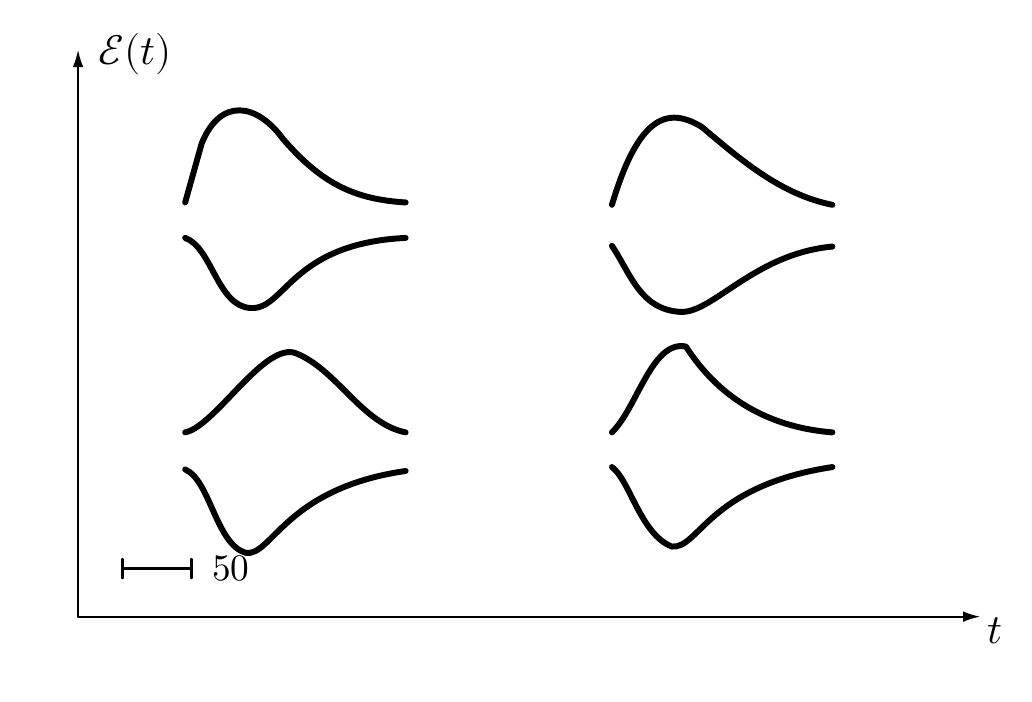
\begin{tikzpicture}[x=1cm,y=1cm,>=Latex,line cap=round,line join=round,font=\fontsize{15}{18}\selectfont]


% Published oscilloscope traces: author-shape reconstruction (NOT raw experimental samples).
\path[use as bounding box] (0,0) rectangle (12.4,8.2);
\draw[axis] (.64,.72)--(12.1,.72);
\draw[axis] (.64,.72)--(.64,7.92);
\node[textlabel,anchor=west] at (.78,7.86) {$\mathscr E(t)$};
\node[textlabel,anchor=west] at (12.07,.54) {$t$};
% Pair geometry follows source: a,b in top row, v,g in bottom row.
\begin{scope}[shift={(2.0,5.98)}]
\node[smalllabel,anchor=east] at (-.28,-.14) {а};
\draw[curve] (0,0)--(.21,.75) .. controls (.45,1.34) and (.91,1.26) .. (1.24,.81) .. controls (1.74,.23) and (2.16,.04) .. (2.80,0);
\draw[curve] (0,-.45) .. controls (.34,-.57) and (.41,-1.32) .. (.83,-1.34) .. controls (1.27,-1.37) and (1.34,-.52) .. (2.8,-.45);
\end{scope}
\begin{scope}[shift={(7.42,5.95)}]
\node[smalllabel,anchor=west] at (3.08,-.18) {б};
\draw[curve] (0,0) .. controls (.34,1.14) and (.71,1.25) .. (1.14,.99) .. controls (1.65,.56) and (2.15,.13) .. (2.8,0);
\draw[curve] (0,-.52) .. controls (.24,-.88) and (.36,-1.33) .. (.87,-1.36) .. controls (1.28,-1.38) and (1.81,-.62) .. (2.8,-.53);
\end{scope}
\begin{scope}[shift={(2.0,3.06)}]
\node[smalllabel,anchor=east] at (-.28,-.12) {в};
\draw[curve] (0,0) .. controls (.39,.08) and (1.02,1.18) .. (1.42,1.0) .. controls (1.94,.78) and (2.25,.11) .. (2.8,0);
\draw[curve] (0,-.47) .. controls (.32,-.61) and (.39,-1.42) .. (.77,-1.53) .. controls (1.1,-1.58) and (1.27,-.71) .. (2.80,-.49);
\end{scope}
\begin{scope}[shift={(7.42,3.06)}]
\node[smalllabel,anchor=west] at (3.08,-.12) {г};
\draw[curve] (0,0) .. controls (.32,.31) and (.51,1.18) .. (.94,1.09) .. controls (1.34,.47) and (1.94,.07) .. (2.8,0);
\draw[curve] (0,-.44) .. controls (.23,-.61) and (.36,-1.29) .. (.76,-1.45) .. controls (1.11,-1.48) and (1.22,-.68) .. (2.8,-.44);
\end{scope}
% 50 ns: source's horizontal scale bar, with perpendicular terminal caps.
\draw[axisplain,line width=1.0pt] (1.20,1.33)--(2.08,1.33);
\draw[axisplain,line width=1.0pt] (1.20,1.21)--(1.20,1.45);
\draw[axisplain,line width=1.0pt] (2.08,1.21)--(2.08,1.45);
\node[smalllabel,anchor=west] at (2.22,1.33) {$50\,\mathrm{нс}$};

\end{tikzpicture}
\end{document}
